\hspace{3em}
GIT est un gestionnaire de version décentralisé. C’est un outil permettant de travailler à plusieurs sur un même projet tout en permettant un suivi contribution par contribution des développeurs. En plus d’être un nouvel outil pour la majorité des membres du groupe, son utilisation peut parfois être contre intuitive. Nous avons alors organisé une petite réunion en début de projet où ceux déjà initiés (Zacharia et Alexis) ont expliqué comment il fonctionnait et ainsi défini certaines normes et bonnes pratiques à respecter.

	La première chose a été d’expliquer le fonctionnement des branches sur git. La principale étant la branche master, nous l’avons directement sécurisée en empêchant les gens d’envoyer directement leurs changements sur celle-ci. Le seul moyen de proposer des modifications est grâce aux merge request (cf partie suivante sur gitlab et son utilité). Chaque développeur tire alors une branche depuis master pour développer les fonctionnalités qu’il souhaite implémenter puis les ajoute à master une fois complétées et validées. Avoir un tel découpage permet un meilleur visuel du travail de chaque développeur et de pouvoir intervenir en cas de problèmes. De plus il permet de ne pas “abîmer” la branche master avec des commits ajoutants des erreurs inaperçues.

	Au niveau des commits nous avons également essayé de garder une unicité au niveau de leur nommage pour y faciliter la navigation. En plus d’avoir essayé au maximum de donner des noms significatifs, nous avons tenté d’appliquer un équivalent simplifié ci-dessous de la convention de nommage utilisée sur le repos git d’Angular (documentation disponible en bibliographie).

git commit -m “<type> (<scope>): <subject>”

Tout le message doit être écrit en minuscule, essayer de ne pas dépasser les 100 caractères au total. Les différents champs du message ont chacun un objectif :

\textbf{type : De quelle façon le commit modifie le projet} (1 mot exactement) parmis les suivants :
\begin{itemize}
  \item \textbf{feat} (feature = nouvelle fonctionnalité)
  \item \textbf{fix} (bug fix)
  \item \textbf{perf} (changement dans le code qui améliore les performances)
  \item \textbf{refactor} (un changement dans le code qui n’ajoute pas de fonctionnalité et ne règle pas de bug non plus)
  \item \textbf{add} (ajout d’un nouveau fichier ou de code qui ne constitue pas une fonctionnalité en soit)
  \item \textbf{test} (ajout de tests)
  \item \textbf{doc} (ajout de documentation)
  \item \textbf{style} (changement qui ne modifie pas le sens du code mais la forme, par ex parenthèses manquantes, pts virgule, …)
\end{itemize}

\textbf{scope : Sur quoi porte le commit} (entre 1 et 3 mots) par exemple :
\begin{itemize}

  \item le nom d’un fichier en particulier
  \item le nom d’un dossier
  \item une fonctionnalité en particulier
  \item une fonction en particulier
\end{itemize}

\textbf{subject : Ce que fait le commit} (max 80 caractères) par exemple :
\begin{itemize}

  \item “ajout d’une fonction de saisie d’un coup”
  \item “ajout batterie de tests sur type position”
  \item “parenthèses manquantes fonctions affichage”
\end{itemize}

\begin{center}
\textbf{On obtient alors un graphe qui a la forme suivante}
\end{center}
\begin{figure}[h]
  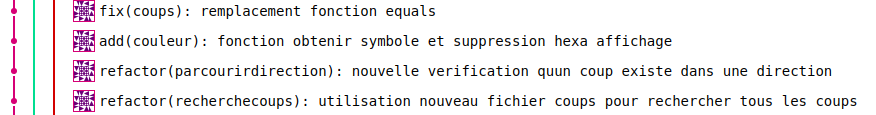
\includegraphics[width=18cm]{./sourcesIMAGES/commits.png}
  \caption{Les messages de commits sont clairs, on sait sur quoi portent les modifications}
\end{figure}
